
    \section{Software choices}
        As we need to build a simulation platform, the first guess would be to use pre-existing physics engines to build our simulation such as PyBullet or Gazeboo framework that are well known in simulation field. The reason why we are building our own simulation framework is because we are not building a physics engine, but rather a mathematical solver for a specific scenario. Also by building our own implementation we can specifically add or removes modules that will analyze simpler or more complex scenarios. We also controls how valid the output is as we knows what hypothesis has been made during the implementation. With those facts, we decided to build our own framework. The choice of the programming language is determined by the tasks we need to achieve, which are characterized by mathematical solver and ease of modular design. This leaves us two main languages, Python and Matlab, both are very similar but Python is well known regarding machine learning tools available and Python would gives us more flexibility in case of future work involving machine learning analysis. Based on those points, we choose Python as a main language. 
    
    \section{Program structure}\label{sec:program_structure}
        Our framework will be built using Python 3. This allows us to create modularity in the structure of the simulation. As we can see on Figure \ref{fig:code_structure}, each physical part of the robot has its own module and implementation. Each module is responsible to respect the physical constraints of its own, to draw the module, to compute displacement given a specific input and to returns different values or points. The modules offer a great flexibility for future improvement or refinement if necessary. We have six modules that represent a simulation: \textit{bar, block, joint, robot, spring, simulation} and a main module that handle the configuration and the environment of the simulation. \\
        
        \begin{figure}
            \centering
            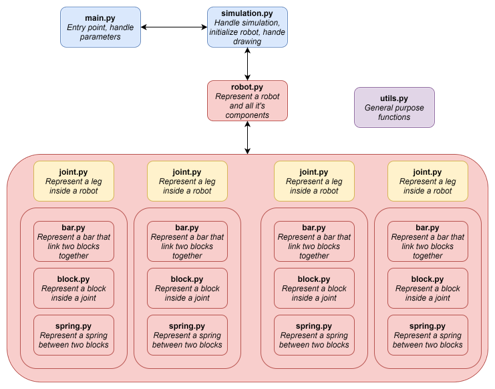
\includegraphics[width=0.8\textwidth]{images/code_structure.png}
            \caption{Caption}
            \label{fig:code_structure}
        \end{figure}
        
        \paragraph{bar}
            module represent the arms in a bistable joint. Those arms are connecting two blocks together with 4 anchors points. It is represented by two low anchors linked to the bottom block and two high anchors linked to the top block. Bar also has a length parameter. It contains functions to draw bars as output and could implement joint friction in the future if needed. 
        \paragraph{block}
            module is the basic structure of the robot, it represents one of the three blocks in the multistable joint. therefore it has a specific width, height, a center of mass location and anchors points to attach the arms. It also handles information about which block it is (bottom, middle, top) and to which actuator it is connected to, in order to have the correct representation while drawing. This module contains functions to compute position of anchors where the arms are linked in addition to the drawing functions.
        \paragraph{joint}
            module represent the multistable structure, composed of three blocks, two springs and four bars. This module allows lots of parameters, such as: joint sequence as seen in section \ref{sec:sequences}, position of the joint relatively to the main frame center of mass, initial position of the joint, arms length ($r_1, r_2$), maximum angle ($\theta_{s1}, \theta_{s2}$) and different colors. This module first initialize the position of the different sub-modules with the input constraints such as maximum angle and arms length. It also contains the different computation parts that animate the legs depending of one of the 15 implemented sequences. Those sequences are based on two simple function that take care of displacing the middle block or the top block. 
        \paragraph{robot}
            module is responsible to build the four multistable joints, the two actuators and the main frame. It contains the joints positions relative to the robot space and coordinate the actuators motions to the multistable joints. The attitude and the position of the robot is also controlled inside this module. Each time the robot is performing a displacement, the module recompute the touching points and the correct orientation of the robot. This module is also responsible of drawing the main frame and the different helps beside the robot such as the orientation of the robot.
        \paragraph{spring}
            module is used today only as a drawing part for the multistable joint. But it can handle future upgrade such as computing forces. 
        \paragraph{simulation}
            module is a top level part that is responsible to ensure the simulation is running smoothly. It receives the different parameters from the main module and create the robot from those. Once the robot initialized, simulation module can start to apply motion to the actuators and to store results of motion of the robot. It is also responsible to aggregate the different output points from the robot module to store them in a Pandas Dataframe which is saved for later use. 
        \paragraph{main}
            module is a very short module that is responsible to load the configuration file that contains the parameters of the simulation and to then load the simulation with this configuration file. 
    \section{Configuration}\label{sec:config}
        As discussed in the appendix section \ref{sec:program_structure}, the simulation is created using a configuration file. This file is use a JSON structure, which is a $key$ $value$ type. There is two main category of settings: \textit{simulation} and \textit{robot}. 
        
        The first one contains the different settings regarding the simulation process, such as \textit{actuation} field that contains the number of steps to compute, the number of cycles to simulate and the phase difference between the actuators. A phase difference of $0$° means that both actuators extend or retract at the same time. A phase difference of $180$° means that while one actuator is extending, the other is retracting itself. \textit{Draw} Boolean determine if there is drawing output produced. It can be useful to set it to false if we want to run the experiment fast and only produce data-points of positions without having a video produced each time. \textit{Camera\_robot\_ref} Boolean allows to have a fixed camera if false or to have the camera that will follow the robot motion if set to true.
        
        The second group of parameters is used to initialize robot's parameters. Each leg can be configured specifically. We have a \textit{sequence} parameter that we can set to one of the 15 sequences encoded (A-O). \todo{Setup the r1 r2 parameters}
        
    \section{Simulation process}
        The simulation process is straightforward. First we initialize the starting point of the robot and the position of each block from the four multistable legs. We also create the actuation matrix regarding the parameters and the physical constraints of the blocks. The actuators are set to run to the maximum position they can reach with the multistable joint. We also dissociate the forward motion from the backward motion, which make it easier later to know what motion to perform depending of the sequence.
        
        Once the initialization is done, we can start the simulation with a loop that will go through all the steps of the simulation. The total number of steps is equal to $cycles \cdot steps$ and for each step we will call a function to update the position of the robot and then draw the updated position. 
        
    \section{Update robot position}
        To update the robot position, the simulation gives first priority to moves the multistable joint individually. Each leg receive the displacement coming from the linked actuator and perform the correct motion of blocks regarding the sequence selected for each sequence. Once the motion from the legs done, we will update the attitude and the position of the robot from the position of the legs.
        We first compute the new attitude of the robot, which is represented by a pitch (y axis) and roll (y axis) rotations. To compute the angle of the robot relative to the ground, we will first sort the legs by their relative high in their own reference frame. Once done we have four possible cases, have one to four legs that are high and so that are touching the floor by default. We can resolve the case in the following way:
            \paragraph{One leg} is touching the floor. As it is not possible to get at equilibrium state on one leg, we need to look for the next leg(s) that will be touching the ground. We know that the gravity will pull the center of gravity of the robot toward the ground but it will go down with an axis of rotation that is located at the touching leg point and the rotation line will be parallel to the ground and perpendicular to the vector going from the touching leg to the center of gravity of the robot. We then look which of the remaining leg require the smallest rotation of the robot to be touching the ground plane. The smallest angle will determine which leg(s) will then also touch the floor. We now have two, three or four touching legs and we move to the specific case respectively.
            \paragraph{Two legs in diagonal} are touching the floor. So here we have either legs one and four that are touching the ground, either legs two and three. This is a specific case where the robot is at an equilibrium state and so we can compute the roll and pitch inclination. 
            \paragraph{Two legs not in diagonal} are touching the floor, in this case, we need to find a third or fourth point off contact. The process is similar than in the one leg case. We have the center of gravity of the robot that will go down and rotate around an axis. This axis is represented by a line going from the two legs that are already touching the floor. We then find the leg that require the smallest angle to touch the ground. We then move to the three legs case or the four legs case if both other legs are touching the floor. 
            \paragraph{Three legs} are touching the floor. To compute the pitch and roll angle, we first define the plane with three legs and compute the angle difference with the flat plane. 
            \paragraph{Four legs} are touching the floor. It is very similar than the three leg process, we just select three legs that will create our plane to compute the roll and pitch.
            \\
            
            Once we know how many legs (and which) are touching the floor, we can start to compute how legs motions translate to robot displacement. To do this we will first compute a ratio number for each leg (displacement ratio). This displacement ratio is equal to zero if the associated leg is not touching the floor as seen in Equation \ref{eq:displacement_ratio}. This can be understood as if a leg is not touching the floor, this leg will not be able to convert its motion to robot's displacement. The sum of the 4 displacement ratio sum to one. Then we compute the distance of the leg to the center of gravity of the robot for each leg. To get the displacement ratio we divide the distance to the center of gravity by the sum of all the distance from legs to the center of gravity of the touching legs.

            \begin{equation}
                displacement\_ratio_i = 
                \begin{cases}
                  leg_i\_dist \left(\sum_{j=1;j=touch}^{n}leg_j\_dist\right)^{-1} & \text{if $leg_i$ is touching the floor}\\
                  0 & \text{otherwise}\\
                \end{cases}  
                \label{eq:displacement_ratio}
            \end{equation}
            
            To get the final displacement of the leg in x-axis and y-axis we multiply the displacement of the leg by its displacement ratio. Then we can sum the displacement of the touching legs to get the robot's displacement.
            To compute the change in orientation of the robot, we proceed similarly. We compute the angle difference of two vectors, the first vector represent the previous position of the leg, the second vector represent the current position of the leg in the robot's reference frame. This angle is computed with Equation \ref{eq:vector_angle}. Once we get all the angles we can multiply them by the same displacement ratio number and sum them to get the total rotation of the robot.

            \begin{equation}
                \phi_i = sng(V_1 \wedge V_2) arctan\left(\frac{\lVert V_1 \wedge V_2 \rVert}{V_1 \cdot V_2}\right)
                \label{eq:vector_angle}
            \end{equation}
            
            We can see that with this method. If two legs are at the same distance from the robot's center of gravity and are doing an equal displacement but in opposite direction, we would have no displacement translated to the robot. If both legs do the same displacement in the same direction, then we would have a displacement of one leg or half the displacement of both legs.

    \section{Displacement mapping}
        We know have a simulation environment that can process different parameters. It is time to create a controller for this multistable-based robot. Before creating the controller we need to get the action our robot can take. To do this we will create a mapping table where each row will contain the following information. The sequence used by the robot, which is represented by four letters, corresponding respectively to sequence for legs one to four. The phase difference of the actuators, which can be in phase, or in opposition of phase (0°, 180°). A boolean that represent a reverse actuation, this term is used to produce symmetric results. Finally we will also have the output of the simulation on each row which corresponds to the displacement in x-axis (in meters), y-axis (in meters) and the change of orientation (in rad) of our robot after one cycle. 
        To create this table we use a specific program (\textit{mapping.py}) that will run through all our realistic sequences (A-J) and run all the possible simulation. This will produce a table off $10^4 \cdot 2 \cdot 2 = 40'000$ rows. Those rows will then be used as input or our controller.
        
    \section{Deep Q-Learning Controller}
        The controller we implemented is a Deep Q-Learning controller which is based in the Reinforcement Learning (RL) principles. It is one of the most popular algorithm in Reinforcement Learning. Reinforcement Learning tackle problems that involve learning how to map situations to actions to maximize a numerical reward signal\cite{sutton_barto}. First, a reinforcement learning task wants to train an agent that is interacting with an environment such as Figure \ref{fig:arena}. In our case, the \textbf{agent} is our robot, and the \textbf{environment} is a surface that contains a goal to reach. The agent is placed in the environment with different scenarios called \textbf{states} and the robot is able to perform \textbf{actions}, in our case the states would be for example the orientation of the robot relative to its goal and the presence of wall in the small signal balls. Also the actions taken from the robot would be the sequence of displacement he choose. Our robot, the agent has one purpose, it is to maximize its total reward across an \textbf{episode} which is completed when reaching to the goal position (large green dot). We reinforce the agent to learn to perform the best actions possible by experience. 
        
        \begin{figure}[h!]
            \centering
            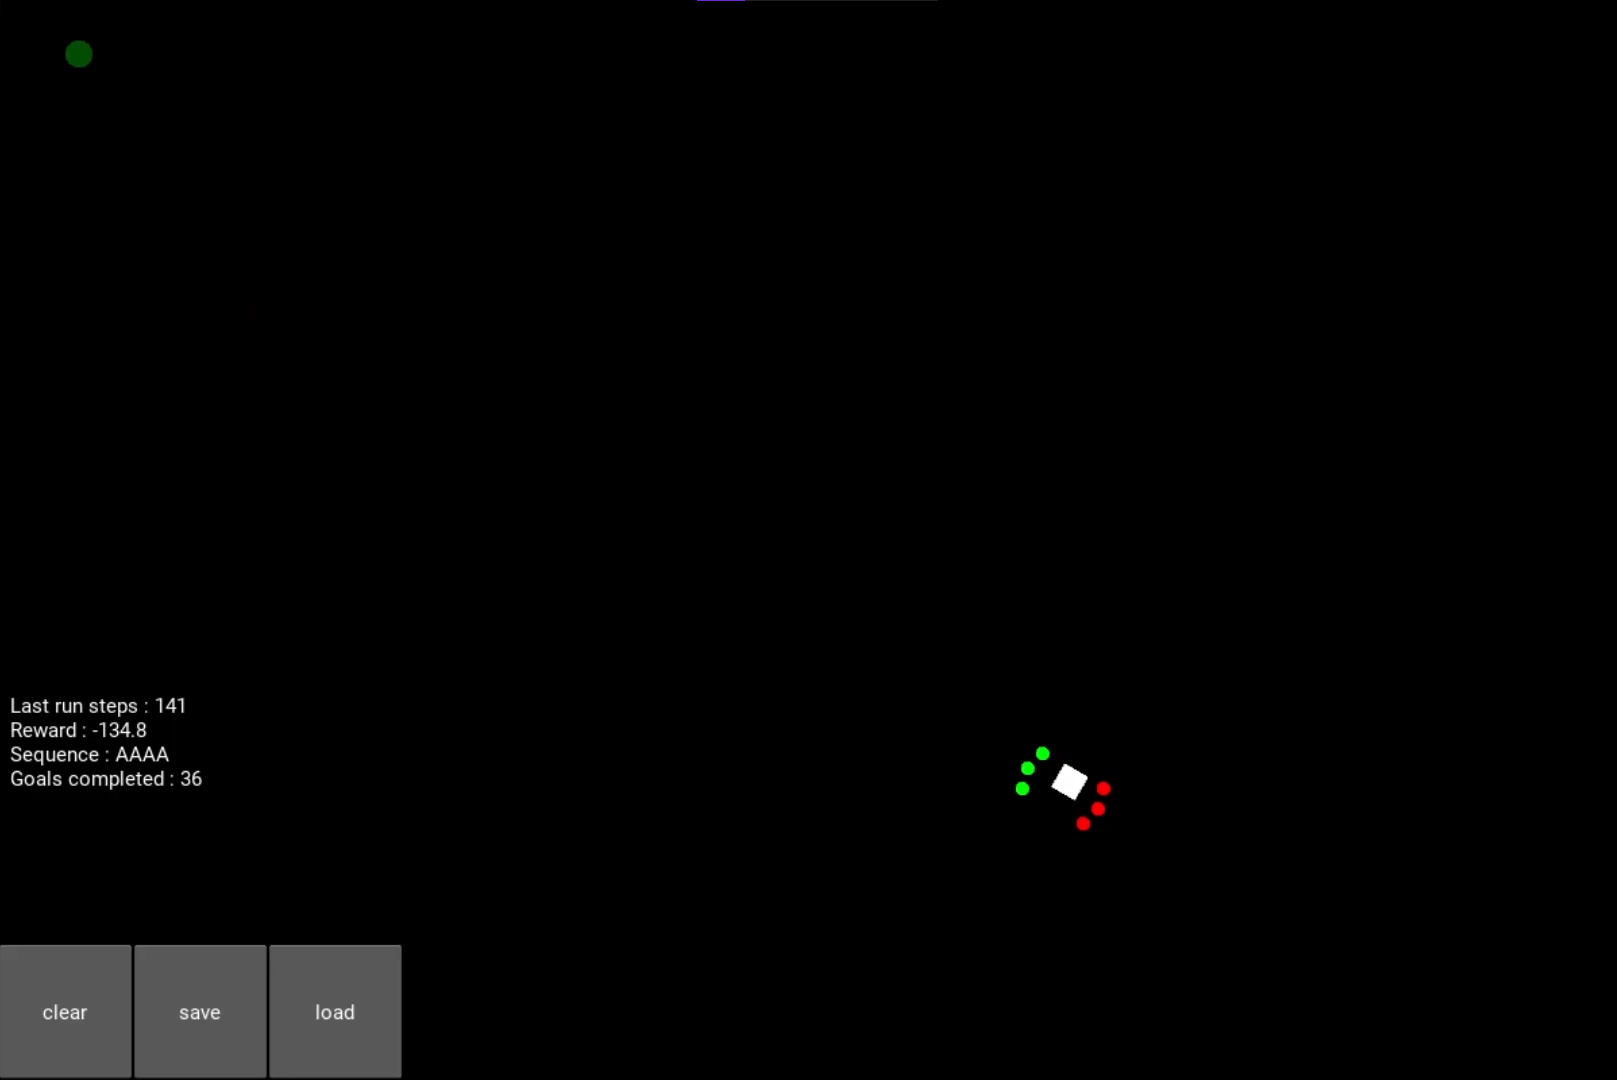
\includegraphics[width=0.66\textwidth]{images/arena.png}
            \caption{Our environment to create a Deep Q-Learning Controller. We can see the robot represented by a white square, it has six sensors, three green sensors in the front, three red sensors in the back. The goal of the robot is represented by a large green dot on the top left. Once the robot reach the goal, a new goal is set. Each step a positive or negative reward is given depending on the consequence of the action taken by the robot.}
            \label{fig:arena}
        \end{figure}
        
        \paragraph{Q Learning}~\\
        If we know the expected reward of each action for every step, we would essentially create a table for the agent and it would be able to understand exactly what action to perform. The agent will perform the sequence of actions that will generate the maximum accumulated reward. This accumulated reward is also called the \textbf{Q-value}. The strategy will be described as Equation \ref{eq:qlearning1} states that Q-value yielded at state $s$ and performing action $a$ is the immediate reward $r(s,a)$ added with the highest Q-value possible from the next state $s'$. Gamma term in the equation is a discount factor which controls the retention of the reward further in the future. As $Q(s',a)$ depends itself from $Q(s'',a)$, Equation \ref{eq:qlearning2} shows the Q-value depending on future states.
        Since this is a recursive equation, we can make arbitrary assumptions for all Q-values. In practical situations, this is implemented as an update equation as shown on Equation \ref{eq:qlearning3}, where alpha is the learning rate and $R$ is the reward.
        
        \begin{equation}
            Q(s,a) = r(s,a) + \gamma \max_{a}Q(s',a)
            \label{eq:qlearning1}
        \end{equation}
        \begin{equation}
            Q(s,a) \rightarrow \gamma Q(s',a) + \gamma^2 Q(s'',a) \dots \gamma^{n} Q(s'^{\dots n}, a)
            \label{eq:qlearning2}
        \end{equation}
        \begin{equation}
            Q(S_t, A_t) \leftarrow Q(S_t, A_t) + \alpha \left[ R_{t+1} + \gamma \max_{a} Q(S_{t+1}, a) - Q(S_t,A_t) \right]
            \label{eq:qlearning3}
        \end{equation}
        
        \paragraph{Deep Q Learning}~\\
        Q-Learning is a simple but already powerful algorithm to create a cheat sheet for our agent. But it can be quickly overwhelmed when the cheat sheet starts to be very long. For example in our environment we have thousands of actions per state and millions of states, this would require a table of billions of cells, which is not practical in reality. We cannot infer the Q-value of new states from already explored states. Therefore, two problems arise, first is the amount of memory required to save and update the table would increase as the number of states increases. Second, the amount of time required to explore each state to create the required table would be unrealistic. The idea of Deep Q Learning is to approximate these Q-values with Machine Learning (ML) models such as a neural network. The state is the input of the neural network and the Q-value of all possible actions is generated as the output. The different steps to create a Deep Q Learning are the following:
        \begin{enumerate}
            \item A memory stores all the past experience
            \item The maximum output of the Q-network determines next action
            \item A loss function compute the error between the predicted Q-value and the target Q-value ($Q^*$). This consists of a regression problem.
        \end{enumerate}
        The target value can be found in Equation \ref{eq:qlearning3} with $R_{t+1} + \gamma \max_a Q(S_{t+1}, a)$. This is a value we don't know as we are dealing with a reinforcement learning problem. The challenge compare to classic Deep Learning methods is that the algorithm is chasing a non stationary target, the training is not stable in a Deep Q Learning method, as it tries to learn to map for a constantly changing input and output.
        
        \paragraph{Our Controller} is using the Deep Q Learning method as the number of states and actions are high. Depending of the sequence the robot is allowed to take we have between $64$ and $202'500$ possible actions. Some filtering to remove duplicate displacement are done to reduce the number of possible action and accelerate the learning process. The neural net used is as simple as possible with an input layer, a hidden layer with 64 nodes and an output layer. The loss function is a Smooth L1 Loss that use the squared term if the absolute element-wise error falls below a threshold and an L1 term otherwise. This function is less sensitive to outliers compare to Mean-Square-Error loss function and prevent gradient exploding problems.
        Signals that are given as input are robot's orientation (positive and negative) relative to the goal and six signals corresponding to the signals of each dots around the robot. Those signals have a value equal to one if they are outside of the environment, zero otherwise. Lastly we give also the reward as input of the neural net. The rewards add up as follow:
        \begin{itemize}
            \item Distance reward:
            \begin{itemize}
                \item A positive reward proportional to the distance improvement compare to the maximum displacement possible during a cycle.
                \item A negative reward proportional to the distance improvement compare to the maximum displacement possible during a cycle.
            \end{itemize}
            \item Orientation reward:
            \begin{itemize}
                \item $+0.2$ when current orientation is better than previous.
                \item $-0.2$ when current orientation is worse than previous.
            \end{itemize}
            \item Action persistence: $+0.02$ when the current action is the same as the previous action. As it takes time to change joint's sequence, we reward the agent when it keep the same sequence during multiple cycles.
            \item Out of bound penalty: $-10$ when the robot is going outside the environment.
            \item Goal reached:
                \begin{itemize}
                    \item A positive reward if number of steps to reach goal is smaller than previous scenario
                    \item A negative reward if number of steps to reach goal is larger than previous scenario
                \end{itemize}
        \end{itemize}
        
            
            